\documentclass[11pt,a4paper]{article}

\usepackage[utf8]{inputenc}
\usepackage[T1]{fontenc}
\usepackage{lmodern}
\usepackage[margin=2.4cm]{geometry}
\usepackage{amsmath,amssymb}
\usepackage{booktabs}
\usepackage{graphicx}
\usepackage{xcolor}
\usepackage{caption}
\usepackage{enumitem}
\usepackage[hidelinks]{hyperref}
\usepackage{fancyhdr}
\usepackage[most]{tcolorbox}

\graphicspath{{figures/}{../figures/}}

\definecolor{accent}{HTML}{A93226}
\definecolor{cool}{HTML}{1F5F8B}
\definecolor{softgrey}{HTML}{F2F4F5}

\newcommand{\var}[1]{\texttt{\small #1}}
\newcommand{\EURMJ}{\ensuremath{\mathrm{EUR}/\mathrm{MJ}}}

% A shaded, unbreakable-where-possible aside. tcolorbox handles the grouping that a
% hand-rolled colorbox+minipage cannot, and allows a page break inside a long one.
\newtcolorbox{keybox}{
  colback=softgrey, colframe=accent, boxrule=0pt, leftrule=2pt,
  sharp corners, breakable, enhanced,
  left=3mm, right=3mm, top=2mm, bottom=2mm, before skip=3mm, after skip=3mm
}

\pagestyle{fancy}
\fancyhf{}
\rhead{\small Fuel market --- step 1}
\lhead{\small AeroMAPS}
\cfoot{\thepage}

\title{\textbf{A clearing fuel market for AeroMAPS}\\[2mm]
\large Step 1: formulation, integration, verification and policy results}
\author{Branch \var{feat/fuel-clearing-step1}}
\date{\today}

\begin{document}
\maketitle

\begin{abstract}
\noindent AeroMAPS is currently \emph{told} the share of each fuel and computes the
resulting cost. This work inverts that: a convex optimisation programme is given a
policy --- an obligation, a penalty, growth limits, capacities --- and returns both the
volume of each fuel produced and the price at which it clears. The programme is solved
once over all regions, all pathways and all prospective years, so it anticipates: it
builds ahead of an obligation it can see coming.

This report states the model in full, describes every parameter, and separates two
classes of result that are easy to confuse: those obtained from the optimisation kernel
\emph{alone}, at a demand fixed from outside, and those obtained with the kernel
\emph{chained into AeroMAPS}, where the price it sets feeds airline costs, airfares and
therefore back into demand. It reports what was verified, what was found to be broken
along the way, and what the mode cannot yet do.

The headline results: with scarcity switched off the new mode reproduces the existing
one to $1.9\times10^{-9}$ across the whole chain; with scarcity on it produces a
quantity AeroMAPS has never had --- a scarcity rent --- and that quantity turns out to
be exactly what makes the coupled fixed point hard to reach.
\end{abstract}

\tableofcontents

\vspace{4mm}
\hrule
\vspace{4mm}

\section{What this is, and what it answers}

The existing AeroMAPS energy chain answers: \emph{given these fuel shares, what does the
scenario cost?} It cannot answer \emph{given this policy, what fuel gets made?}, because
the quantity produced in response to a policy is exactly what a market determines and
the current model is handed it as an input.

The fuel market adds a second mode, opt-in and default off. Both modes coexist; they
answer different questions. The new one takes an obligation, a penalty for missing it,
a production cost and a set of physical limits per pathway, and returns:

\begin{itemize}[nosep,leftmargin=*]
  \item \textbf{volumes} --- how much of each fuel is produced, in each region, each year;
  \item \textbf{prices} --- what the energy is worth at the margin, what the obligation
        costs to comply with, and what a growth limit is worth relaxing.
\end{itemize}

The prices are not assumed or calibrated. They are the Lagrange multipliers of the
programme's constraints, which is what makes convexity worth paying for: a convex
programme has one optimum, and its multipliers are certified prices that do not depend
on where the solver started.

\section{The model}
\label{sec:model}

\subsection{The programme}

Over regions $r \in \{1..R\}$, pathways $p \in \{1..P\}$ and prospective years
$t \in \{1..T\}$, with decision variables $q_{r,p,t} \ge 0$ (energy produced, MJ) and
$x_{r,t} \ge 0$ (obligation released by paying the penalty, MJ):

\begin{equation}
\min_{q,\;x}\;\; \sum_{t} \delta_t \left[
  \sum_{r,p} \underbrace{\left( c_{r,p,t}\, q_{r,p,t}
    + \frac{c_{r,p,t}\,\gamma_{r,p}\,K_{r,p,t}}{n+1}
      \left(\frac{q_{r,p,t}}{K_{r,p,t}}\right)^{n+1} \right)}_{\text{production cost, integral of the marginal cost}}
  \;+\; \sum_{r} B_{r,t}\, x_{r,t}
\right]
\label{eq:objective}
\end{equation}

subject to, for every region $r$ and year $t$:

\begin{align}
\sum_{p} q_{r,p,t} &= D_{r,t}
  && \text{energy balance} && \to \lambda^{E}_{r,t} \label{eq:balance}\\[1mm]
\sum_{p \in \mathcal{S}_r} q_{r,p,t} + x_{r,t} &\ge m_{r,t}\, D_{r,t}
  && \text{obligation} && \to \lambda^{M}_{r,t} \label{eq:mandate}\\[1mm]
\sum_{p \in \mathcal{N}_r} q_{r,p,t} + x^{\mathrm{sub}}_{r,t} &\ge \mu_{r,t}\, D_{r,t}
  && \text{sub-obligation} && \to \lambda^{S}_{r,t} \label{eq:submandate}\\[1mm]
q_{r,p,t} &\le s_{r,p} + (1+g_{r,p})\, q_{r,p,t-1}
  && \text{growth limit} && \to \lambda^{R}_{r,p,t} \label{eq:rampup}
\end{align}

with $q_{r,p,0} \equiv q^{\mathrm{init}}_{r,p}$ given. $\mathcal{S}_r$ is the set of
pathways \emph{eligible} for region $r$'s obligation and $\mathcal{N}_r \subseteq
\mathcal{S}_r$ the narrower set for its sub-obligation.

Three properties of this programme carry the design.

\begin{keybox}
\textbf{One solve, not one per year.} Constraint~\eqref{eq:rampup} ties $t$ to $t-1$, so
solving year by year would discard anticipation. Sustainable output above the obligation
in early years is a \emph{result}, not an artefact: with perfect foresight the cheapest
way to meet a step is to be ready before it arrives.

\textbf{Convex, so the multipliers are prices.} $\lambda^{E}$ \emph{is} the marginal cost
of energy; $\lambda^{M}$ \emph{is} the compliance price. A fixed point found by
iteration would not come with that guarantee.

\textbf{The growth limit is a sum, not a maximum} (\S\ref{sec:convexity}).
\end{keybox}

\subsection{Every parameter}
\label{sec:parameters}

\begin{table}[h]
\centering\small
\begin{tabular}{@{}llp{8.3cm}@{}}
\toprule
\textbf{Symbol} & \textbf{Shape, unit} & \textbf{Meaning and provenance} \\
\midrule
$D_{r,t}$ & $(R,T)$, MJ & Drop-in energy demand. In coupled mode this is
  \var{energy\_consumption\_dropin\_fuel}, an output of the fleet chain --- which is
  what makes the market part of a loop. \\
$c_{r,p,t}$ & $(R,P,T)$, \EURMJ & Production cost per unit energy at zero utilisation.
  Taken as \var{\{p\}\_net\_mfsp}: the cost the buyer actually faces, carbon tax and
  subsidies included (\S\ref{sec:netgross}). Flat in time on the bench --- AeroMAPS has
  no learning curve, so all price dynamics come from the model, not the supply curve. \\
$m_{r,t}$ & $(R,T)$, fraction & The obligation: minimum eligible share of demand. A
  \emph{fraction}, not a percentage --- validated, because a silent factor of 100 here
  would be invisible downstream. \\
$\mathcal{S}_r$ & $(R,P)$, boolean & \textbf{Eligibility}, not chemistry: which pathways
  count towards region $r$'s obligation. The same fuel may count in one jurisdiction and
  not another. \\
$\mu_{r,t},\ \mathcal{N}_r$ & $(R,T)$, $(R,P)$ & Sub-obligation and its narrower
  eligible set --- ReFuelEU's synthetic-fuel target. Optional; absent by default. \\
$B_{r,t}$ & $(R,T)$, \EURMJ & Penalty (``buy-out'') per unit of unmet obligation. Caps
  $\lambda^{M}$: nobody pays more to comply than to not comply. Without it an
  unreachable obligation makes the programme \emph{infeasible} rather than expensive. \\
$K_{r,p,t}$ & $(R,P,T)$, MJ & Capacity \emph{scale}, not a cap: the output at which the
  pathway starts to strain. $\infty$ disables saturation. Exogenous at step~1. \\
$\gamma_{r,p}$ & $(R,P)$ & Saturation intensity --- how much dearer the next unit is at
  full utilisation. $0$ switches the term off entirely. \\
$n$ & scalar $\ge 0$ & Saturation stiffness --- how \emph{abruptly} the extra cost
  arrives. $n \to \infty$ recovers a hard cap, which is what the soft form exists to
  avoid. \\
$g_{r,p}$ & $(R,P)$, /year & Growth limit: relative expansion allowed year on year. \\
$s_{r,p}$ & $(R,P)$, MJ & Growth \emph{seed}. Not optional in practice: with
  $q^{\mathrm{init}} = 0$ and $s = 0$, \eqref{eq:rampup} pins the pathway at zero
  forever. Not a free dial either --- it is Eq.~(12)'s volume branch
  (\S\ref{sec:convexity}). \\
$q^{\mathrm{init}}_{r,p}$ & $(R,P)$, MJ & Production in the last historical year; the
  growth limit's initial condition. \\
$\delta_t$ & scalar & Discount factor $(1+\rho)^{-t}$. Decides how far ahead of a step
  it is worth building. \\
$w$ & scalar $\in [0,1]$ & \textbf{Pricing weight.} Decides who keeps the scarcity rent
  (\S\ref{sec:whopays}). The single most consequential parameter. \\
\bottomrule
\end{tabular}
\caption{Inputs. $R$ regions, $P$ pathways, $T$ prospective years.}
\end{table}

\subsection{The prices the model produces}

\begin{table}[h]
\centering\small
\begin{tabular}{@{}llp{9.2cm}@{}}
\toprule
\textbf{Symbol} & \textbf{From} & \textbf{Reads as} \\
\midrule
$\lambda^{E}_{r,t}$ & \eqref{eq:balance} & What the next unit of energy costs. Set by
  whichever pathway is on the margin. \\
$\lambda^{M}_{r,t}$ & \eqref{eq:mandate} & What one more unit of obligation costs.
  Bounded above by $B$. \textbf{Zero in any year where the market is already ahead of
  the obligation} --- a slack constraint costs nothing. \\
$\lambda^{S}_{r,t}$ & \eqref{eq:submandate} & The same, for the narrower target. \\
$\lambda^{R}_{r,p,t}$ & \eqref{eq:rampup} & What it would be worth to be allowed to grow
  faster. Zero where the limit is not in the way. \\
\bottomrule
\end{tabular}
\end{table}

\noindent The \emph{marginal price} of a pathway aggregates the constraints one unit of
it relaxes:
\begin{equation}
\mathrm{MC}_{r,p,t} \;=\; \lambda^{E}_{r,t}
  \;+\; \lambda^{M}_{r,t}\,\mathbf{1}[p \in \mathcal{S}_r]
  \;+\; \lambda^{S}_{r,t}\,\mathbf{1}[p \in \mathcal{N}_r].
\label{eq:marginal}
\end{equation}
A sub-mandated unit carries both obligation multipliers. That is not double counting: it
genuinely relaxes two distinct constraints.

\subsection{What the airline actually pays}
\label{sec:whopays}

\emph{This section answers a question the earlier write-ups left implicit.}

Two prices exist for each pathway and they are not the same. The \textbf{average cost}
is what the fuel produced actually cost, per unit:
\begin{equation}
\mathrm{AC}_{r,p,t} = c_{r,p,t}\left(1 + \frac{\gamma_{r,p}}{n+1}
  \left(\frac{q_{r,p,t}}{K_{r,p,t}}\right)^{n}\right),
\end{equation}
against the marginal price \eqref{eq:marginal}. The gap between them is
\textbf{inframarginal rent} --- profit earned on every unit produced more cheaply than
the last one. The pricing weight interpolates:
\begin{equation}
\boxed{\;\mathrm{mfsp}^{\mathrm{mkt}}_{r,p,t}
  = (1-w)\,\mathrm{AC}_{r,p,t} + w\,\mathrm{MC}_{r,p,t}
  \;-\;\underbrace{\left(\mathrm{net}_{r,p,t}-\mathrm{gross}_{r,p,t}\right)}_{\text{tax wedge, \S\ref{sec:netgross}}}\;}
\label{eq:marketmfsp}
\end{equation}
and AeroMAPS's existing machinery then weights that across pathways into the one number
the airline sees, \var{\{type\}\_mean\_mfsp} $= \sum_p \mathrm{share}_{p}\cdot
\mathrm{mfsp}^{\mathrm{mkt}}_{p}$, which drives operating cost, airfare and demand.

\begin{keybox}
\textbf{So: fuel cost, or compliance, or both?} The honest answer is \emph{both, always}
--- but not by addition, and this is the easiest thing in the model to get wrong.

\medskip
\begin{center}\small
\begin{tabular}{@{}lrrr@{}}
\toprule
\textbf{Region A, 2050} & \textbf{Airline pays} & $\lambda^{M}$ & \textbf{SAF share} \\
\midrule
No obligation at all & 0.01200 & 0 & 0\,\% \\
70\,\% obligation, $w=0$ & \textbf{0.01982} & 0.01117 & 70\,\% \\
70\,\% obligation, $w=1$ & 0.01982 & 0.01117 & 70\,\% \\
\;+ scarcity, $w=0$ & 0.02115 & 0.07917 & 70\,\% \\
\;+ scarcity, $w=1$ & \textbf{0.06742} & 0.07917 & 70\,\% \\
\bottomrule
\end{tabular}
\end{center}
\medskip

\textbf{The obligation is paid for at $w=0$}: the bill goes from $0.01200$ to
$0.01982$, \textbf{a 65\,\% increase}. It is paid through the \emph{mix} --- the
obligation forces 70\,\% of the fuel to be the expensive kind --- not through a separate
charge. The cost of compliance is \emph{embedded}, not itemised.

\textbf{$\lambda^{M}$ is not added on top of that, and must not be.} It is the
\emph{marginal} cost of the obligation --- what one more unit of it would cost. The
average cost increment is $0.01982-0.01200 = 0.00782$, which is exactly
$0.70 \times \lambda^{M}$: share times marginal cost. Adding $\lambda^{M}$ to the
delivered price would give $0.03099$, a 158\,\% increase, \textbf{charging the obligation
twice}.

\textbf{What $w$ changes is average versus marginal, not paid versus unpaid.} At $w=1$
every unit is priced at the \emph{last} unit's cost. With nothing scarce that is the same
number (rows 2 and 3 are identical --- marginal equals average when the supply curve is
flat). With scarcity it is not: $0.06742$ against $0.02115$, and the difference is
inframarginal rent.

\textbf{It is never ``compliance only''.} $\lambda^{M}$ is a premium on top of the energy
price, never a substitute for it.

\textbf{The carbon tax} arrives separately, as its own \var{DirectOperatingCosts} line
--- which is exactly why \eqref{eq:marketmfsp} subtracts the tax wedge back out
(\S\ref{sec:netgross}). Same double-counting logic, different instrument.
\end{keybox}

\begin{keybox}
\textbf{One thing the airline does \emph{not} pay, and arguably should.} The buy-out
payment $B\,x$ appears in objective~\eqref{eq:objective} but in no price output. If the
market releases part of the obligation, that penalty is borne by nobody in the cost
chain. At $w=1$ the \emph{rate} is signalled correctly ($\lambda^{M}$ is capped at $B$),
but the \emph{payment} is not accounted anywhere. This is a known gap, not a modelling
choice.
\end{keybox}

A useful consistency check falls out: with no scarcity at all, $\lambda^{E} = c_{k}$
(kerosene) and $\lambda^{M} = c_{s} - c_{k}$, so a sustainable pathway's marginal price
is exactly $c_{s}$ --- which is also its average cost. The two endpoints of
\eqref{eq:marketmfsp} coincide and $w$ is inert. \textbf{$w$ only matters where something
is scarce}, from \emph{either} the capacity term or a binding growth limit.

\subsection{Two choices that keep the problem convex}
\label{sec:convexity}

\paragraph{Capacity squeezes, it does not wall.} Production is not capped. Instead the
marginal cost rises with utilisation, $c\,(1+\gamma(q/K)^{n})$, whose integral appears in
\eqref{eq:objective}. A hard cap would make the price jump discontinuously at $q=K$; since
that price feeds airfares, which feed demand, which feeds fuel demand, a jumping price
makes the coupled loop oscillate instead of settle. Figure~\ref{fig:sat} shows the shape
and the rent.

\begin{figure}[h]
\centering
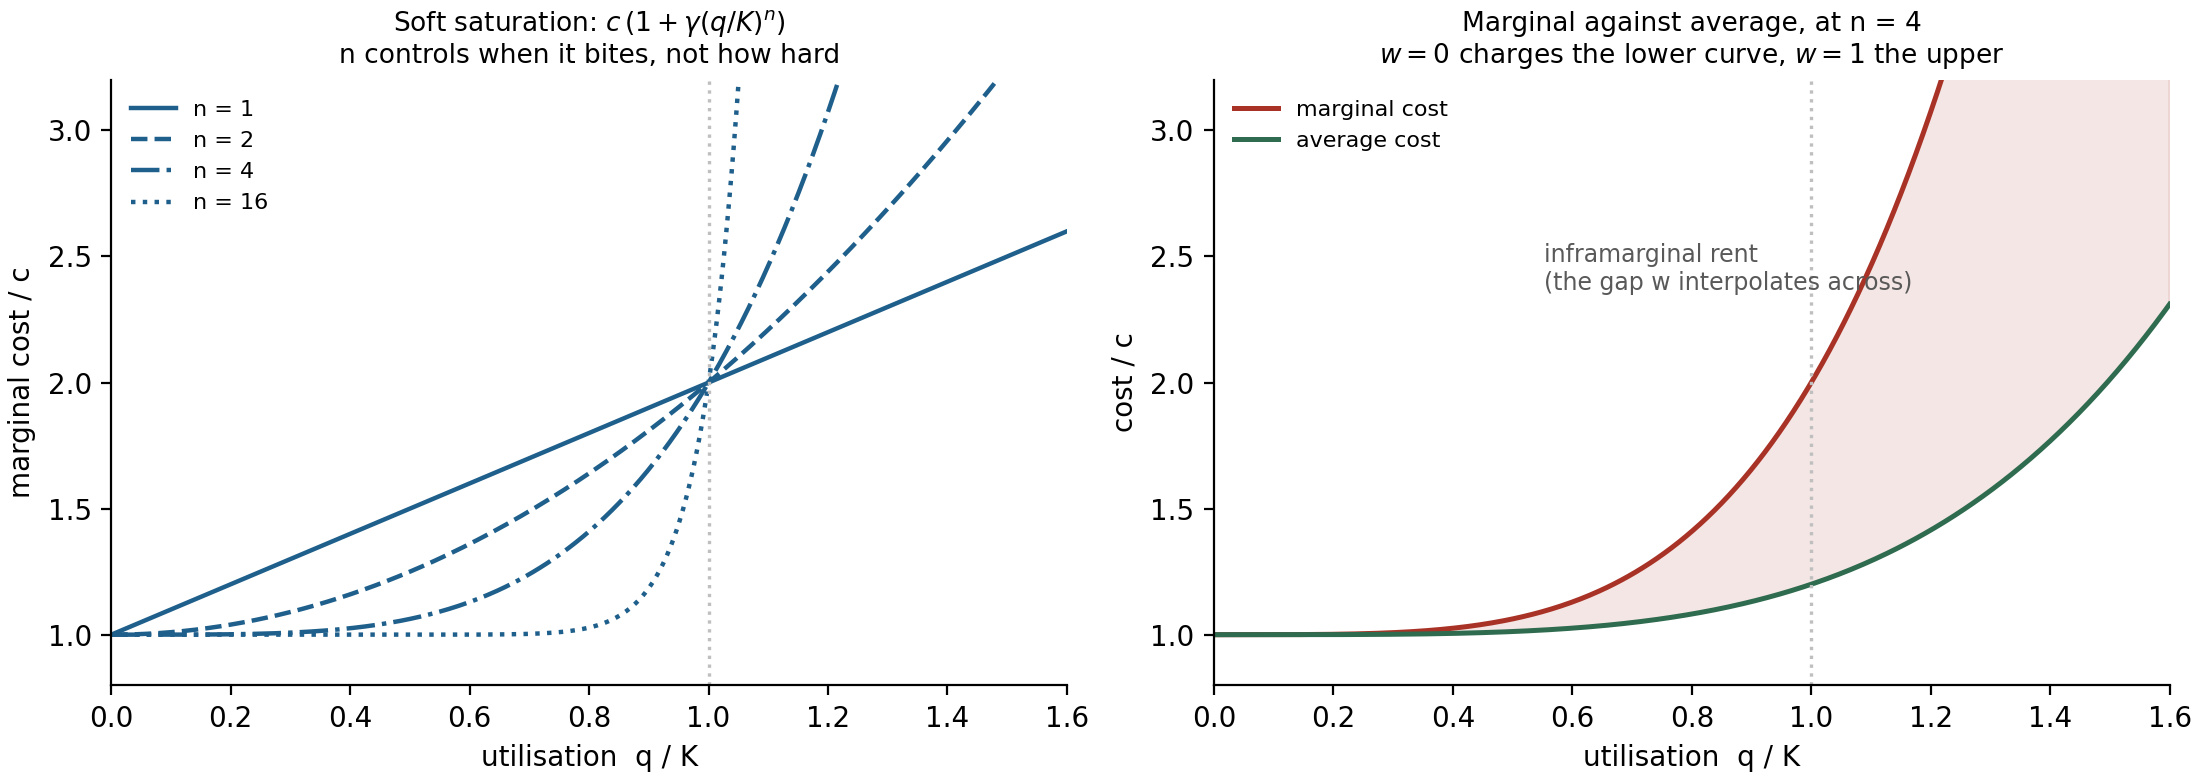
\includegraphics[width=\linewidth]{explain_saturation.png}
\caption{Left: $n$ decides \emph{when} the squeeze bites, not how hard. Note the
consequence --- below $q=K$ a \emph{larger} $n$ gives a \emph{smaller} markup, which is
why stiffness reduces the price on a bench running under capacity. Right: the gap between
marginal and average cost is the rent that $w$ interpolates across.}
\label{fig:sat}
\end{figure}

\paragraph{The growth limit has to be a sum.} AeroMAPS's optimisation mode limits growth
by Eq.~(12) of the published work --- the \emph{more permissive} of a relative rate and a
fixed volume addition:
\begin{equation}
E_t \;\le\; \max\{\, (1+\tau)\,E_{t-1},\;\; E_{t-1} + \Delta E \,\}.
\label{eq:eq12}
\end{equation}
The region under a maximum of two affine functions is not a convex set
(Figure~\ref{fig:ramp}, right), so \eqref{eq:eq12} cannot be handed to a convex solver.
This is not a tolerance problem; the feasible set is the wrong shape.
Constraint~\eqref{eq:rampup} replaces the maximum with a \emph{sum}, which is its convex
outer relaxation: it admits everything \eqref{eq:eq12} admits, plus a margin
\textbf{measured at 0.73\,\%, independent of $g$}.

\begin{figure}[h]
\centering
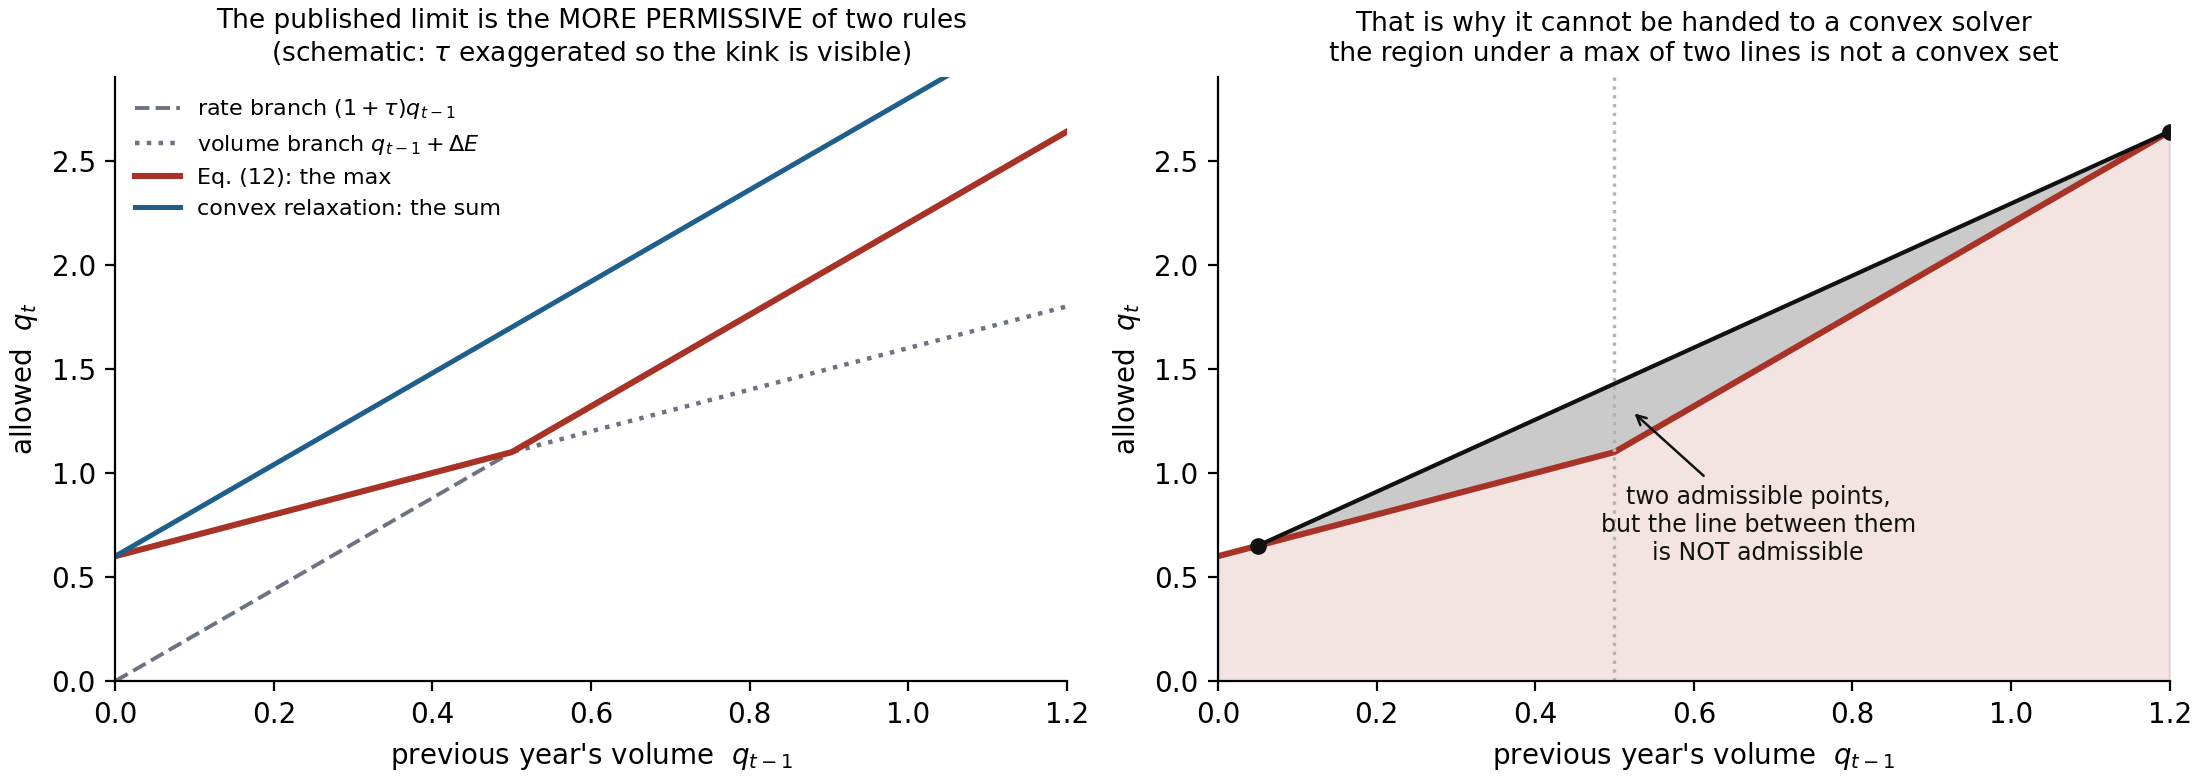
\includegraphics[width=\linewidth]{explain_rampup.png}
\caption{Why the published growth limit cannot go into the programme, and what replaces
it. Right: two admissible points whose connecting line is inadmissible --- the definition
of a non-convex set.}
\label{fig:ramp}
\end{figure}

\noindent The seed $s$ in \eqref{eq:rampup} is Eq.~\eqref{eq:eq12}'s volume branch
$\Delta E$, so it is \emph{not} a free parameter: the published calibration
($0.2$\,EJ/yr at an ASK share of $0.1549$) puts it at about \textbf{1.5\,\% of annual
demand}. It matters --- on the bench the seed moves the compliance price by a factor
$4.3$ across a plausible range.

\section{How it plugs into AeroMAPS}

\subsection{Two levels of result, and why the distinction matters}
\label{sec:twolevels}

\emph{This section answers the second question the earlier write-ups left implicit.}

Results in this report come from one of two set-ups, and conflating them would be a
serious misreading.

\begin{table}[h]
\centering\small
\begin{tabular}{@{}p{4.2cm}p{5.4cm}p{5.4cm}@{}}
\toprule
 & \textbf{Kernel only} & \textbf{Chained into AeroMAPS} \\
\midrule
What runs & The convex programme alone. NumPy arrays in, arrays out. No AeroMAPS import.
  & The programme as a GEMSEO discipline inside the full multi-regional MDA. \\
Demand $D_{r,t}$ & \textbf{Fixed from outside} --- taken from a stored reference run.
  & \textbf{An output of the model}, responding to the price the market sets. \\
Loop closed? & No. Price has no effect on demand. & Yes: price $\to$ operating cost
  $\to$ airfare $\to$ elasticity $\to$ demand $\to$ price. \\
Cost per case & $\sim$0.03\,s & minutes \\
Used for & Formulation, verification, parameter sweeps, \textbf{all policy cases}. &
  Reproduction end-to-end, convergence, the coupled grid. \\
\bottomrule
\end{tabular}
\caption{The two levels. Everything in \S\ref{sec:kernelresults} and \S\ref{sec:policy}
is kernel-only; everything in \S\ref{sec:coupledresults} is coupled.}
\label{tab:levels}
\end{table}

\begin{keybox}
\textbf{Why the policy cases are kernel-only, deliberately.} Chaining scales every price
effect by roughly a tenth (\S\ref{sec:coupledgrid}) and changes no \emph{ordering} at
$w=0$, while costing minutes per case --- and at $w>0$ it introduces a convergence
problem (\S\ref{sec:convergence}) that would sit between the reader and the policy
question. The kernel-level results are therefore the \emph{policy} answer; the coupled
results are what tells you how much of it survives the demand response.
\end{keybox}

\begin{figure}[h]
\centering
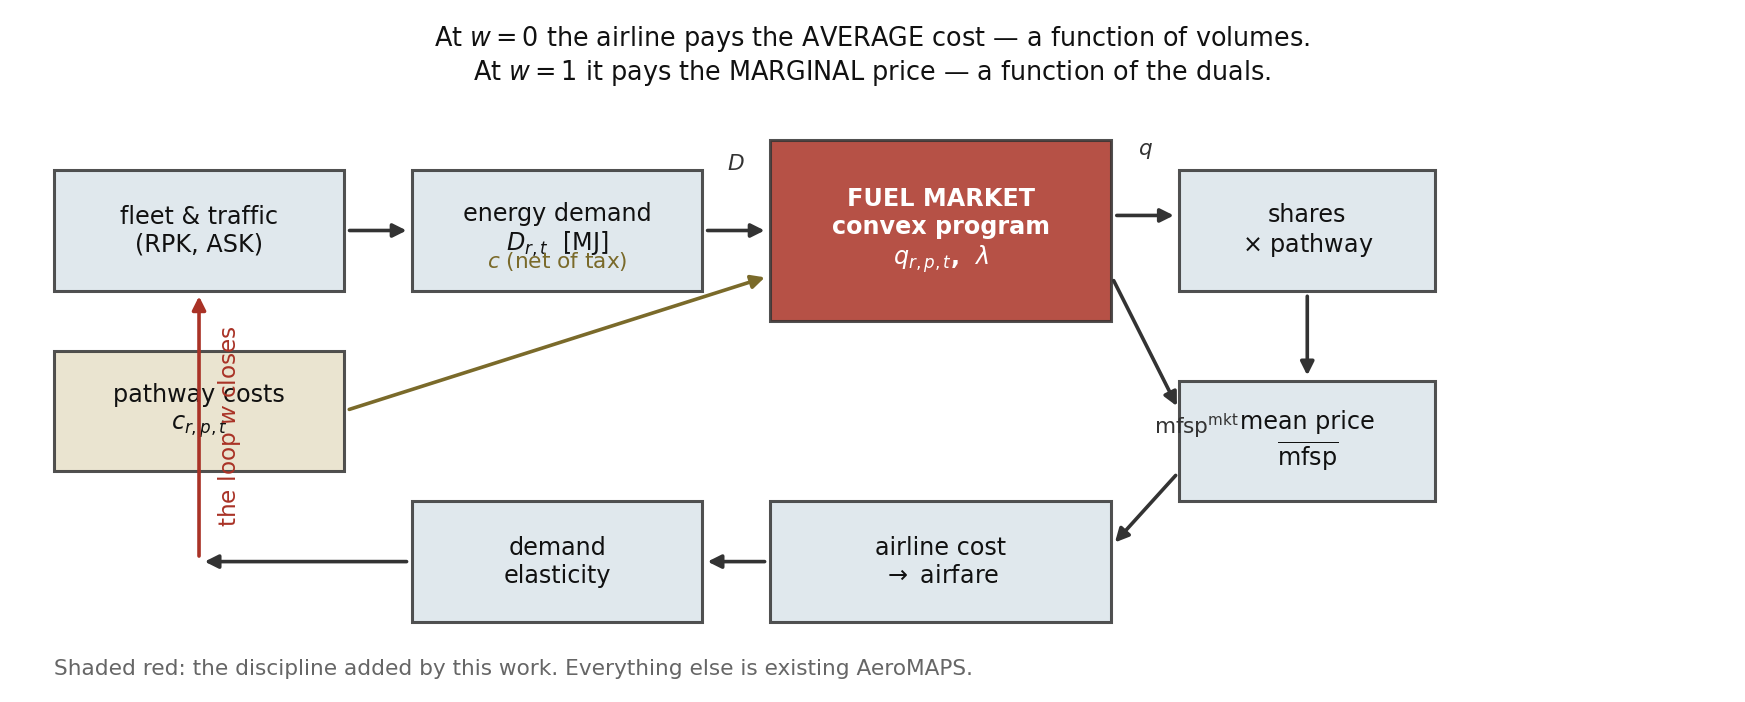
\includegraphics[width=0.94\linewidth]{explain_chain.png}
\caption{Where the market sits. Shaded: the discipline added by this work. The loop on
the left is closed only in coupled mode, and only carries a discontinuous quantity when
$w>0$.}
\label{fig:chain}
\end{figure}

\subsection{What the discipline replaces}

In market mode the existing allocator \var{EnergyUseChoice} is \textbf{not instantiated}:
the market decides the volumes rather than being handed shares. It emits the same nine
output families under the same names, computed by a \emph{shared} function extracted from
the allocator rather than a second copy --- two copies would drift, and the failure is
silent, since a share family disagreeing with its volumes rescales CO$_2$ with no error
raised.

The mode is one configuration key, default off, propagated to each region as a
process-level keyword. It is refused outside the unified-MDA execution mode, and three
guards raise at set-up rather than producing plausible-looking numbers: drop-in fuels
only, top-down cost model only, exactly one residual pathway.

\subsection{Decide on net, report on gross}
\label{sec:netgross}

The market chooses using \var{net\_mfsp} --- cost \emph{including} carbon tax and
subsidies --- because that is what determines which pathway is marginal. This is not
cosmetic: on the bench a carbon tax of only 5\,EUR/t already narrows the sustainable
premium by 3\,\%, and extrapolating the emission factors the premium reaches zero near
\textbf{164\,EUR/t}, where the ordering reverses and the market buys sustainable fuel
unprompted. A market clearing on gross cost could never produce that.

But \var{DirectOperatingCosts} adds the carbon tax as its own line. Publishing a
net-basis price would count the tax twice --- hence the wedge subtracted in
\eqref{eq:marketmfsp}. \textbf{Decide on net, report on gross, and the tax is counted
once.}

A \emph{passenger}-level tax is deliberately excluded from the objective: it is uniform
across fuels, so it cannot change which pathway is marginal. It still reaches the market
through demand, which is the correct channel.

\section{Verification}

\paragraph{An analytic case pins the conventions.} One region, one year, saturation known
in closed form, so both prices are known exactly. This caught a sign error that
documentation could not have: cvxpy reports the equality's multiplier negated, so the
energy price came out as $-0.012$ against an expected $+0.012$ --- a plausible number with
the wrong sign.

\paragraph{38 kernel tests}, covering the balance, the obligation, the growth limit,
scale invariance, continuity and input hygiene.

\paragraph{Complementary slackness, across seven regimes.} A multiplier may be non-zero
only where its constraint is tight. This single property is what all three real defects
(\S\ref{sec:defects}) violated, and nothing tested it. It is now parametrised over the
\emph{edges} --- zero obligation, full obligation, a constraint that cannot bind --- because
a mid-range case sees none of them. Worst residual: $1.4\times10^{-8}$, solver noise; the
phantom compliance price scored $0.46$ on the same measure.

\section{Results without the chain (kernel only)}
\label{sec:kernelresults}

\subsection{It reproduces the current allocator}
Given the reference run's shares, with saturation off and the growth limit loose, the
market lands on the reference allocation with a residual below $10^{-8}$ of demand --- an
order of magnitude under solver noise.

\subsection{Perfect foresight builds ahead of the obligation}
At $g = 15\,\%$/yr against the ReFuelEU steps, region A holds \textbf{more} sustainable
fuel than it owes in every year between steps: 14.1\,\% in 2034 against a 6\,\%
obligation, 28.9\,\% in 2039 against 20\,\%. The growth limit cannot take it from 6\,\% to
20\,\% in the year the step lands, so it starts early. Sustainable fuel is the expensive
option and discounting penalises early spend, so it overshoots by the \emph{minimum} that
clears the next step --- which is what a firm reading a published mandate would do.

The penalty is needed exactly once, at the 2035 step and only at the tightest growth
limit. The compliance price is \textbf{zero in every year where the market is ahead}.

\subsection{Which parameters move the answer}

\begin{table}[h]
\centering\small
\begin{tabular}{@{}lll@{}}
\toprule
\textbf{Parameter} & \textbf{Swept} & \textbf{Spread in delivered price} \\
\midrule
Pricing weight $w$ & 0 $\to$ 1 & \textbf{37.3\,\%} \\
Stiffness $n$ & 1 $\to$ 16 & \textbf{16.3\,\%} \\
Penalty $B$ & 0.02 $\to$ 0.30 & \textbf{8.3\,\%} \\
Growth limit $g$ & 0.10 $\to$ 1.20 /yr & 3.8\,\% \\
Intensity $\gamma$ & 0 $\to$ 4 & 1.7\,\% \\
Discount rate $\rho$ & 0 $\to$ 0.08 & 0.0\,\% \\
\bottomrule
\end{tabular}
\end{table}

\noindent Two readings that a single-parameter view gets wrong. \textbf{$\gamma$'s
1.7\,\% is misleading}: it was measured at one stiffness, and at $n=1$ the same range
moves the uplift 4\,\%$\to$16\,\%. The two saturation parameters are not separable. And
$\gamma$'s real effect at this baseline is on the \emph{compliance} price, which it moves
$+57\,\%$ --- scarcity raises the cost of the obligation well before it raises the average
fuel bill.

\textbf{The penalty is inert until it is cheap enough to be worth paying.} The
obligation's own marginal cost here is $0.0546$\,\EURMJ. Set $B$ above that and it never
binds; set it below and the market stops building and pays instead, and the
\emph{delivered} price falls 8.3\,\%. A penalty priced under the cost of compliance is a
subsidy to non-compliance.

\subsection{Capacity sized on the obligation is undersized}
With a binding growth limit, anticipation pushes utilisation to $q/K = 2.01$ between
steps: the market builds twice the plant the obligation asks for. Saturation disciplines
it --- at $\gamma=1$ the peak falls to $1.30$.

\section{Results with the chain (coupled)}
\label{sec:coupledresults}

\subsection{End-to-end reproduction}
With nothing scarce, the coupled mode must reproduce the existing model. It does, and not
only in the volumes:

\begin{table}[h]
\centering\small
\begin{tabular}{@{}lrrr@{}}
\toprule
\textbf{2050, both regions} & \textbf{reference} & \textbf{market} & \textbf{worst rel., all years} \\
\midrule
\var{hefa\_fog\_energy\_consumption} & 9.84171e12 & 9.84171e12 & 1.1e-09 \\
\var{hefa\_fog\_share\_dropin\_fuel} & 70 & 70 & 1.9e-09 \\
\var{dropin\_fuel\_mean\_mfsp} & 0.019819 & 0.019819 & 1.8e-10 \\
\var{dropin\_fuel\_mean\_co2\_emission\_factor} & 41.1 & 41.1 & 1.0e-09 \\
\var{co2\_emissions\_passenger} & 493.04 & 493.04 & 6.3e-10 \\
\var{airfare\_per\_rpk} & 0.0867286 & 0.0867286 & 5.1e-11 \\
\var{rpk} & 1.98233e13 & 1.98233e13 & 1.6e-11 \\
\bottomrule
\end{tabular}
\caption{Worst relative difference across every variable and year: $\mathbf{1.9\times10^{-9}}$.}
\end{table}

\noindent An independent confirmation fell out: the compliance price came back at
$0.01083$, which is the \emph{net}-basis premium ($0.010830$) and not the gross one
($0.011170$). The decide-on-net rule is doing what it claims.

\subsection{Scarcity reaches the traffic loop}

\begin{table}[h]
\centering\small
\begin{tabular}{@{}lrrr@{}}
\toprule
 & \textbf{no scarcity} & \textbf{scarce, $w=0$} & \textbf{scarce, $w=1$} \\
\midrule
Delivered price 2050 & 0.019819 & 0.021839 ($+10.2\,\%$) & 0.04020 (\textbf{$+103\,\%$}) \\
Max compliance price & 0.01083 & 0.047886 & --- \\
RPK 2050 & 1.98233e13 & $-1.2\,\%$ & \textbf{$-10.8\,\%$} \\
CO$_2$ 2050 & 493.04 & $-1.2\,\%$ & --- \\
\bottomrule
\end{tabular}
\end{table}

\noindent Expensive fuel makes tickets dearer and some journeys do not happen. AeroMAPS
could not previously produce that chain of consequences \emph{from a fuel policy},
because nothing in it priced scarcity.

\subsection{The coupled saturation grid}
\label{sec:coupledgrid}

Swept through the full MDA, so volumes respond. Delivered price \% / RPK \% against the
no-scarcity run:

\begin{table}[h]
\centering\small
\begin{tabular}{@{}lrrrr@{}}
\toprule
 & $n=2$ & $n=4$ & $n=8$ & $n=16$ \\
\midrule
$w=0,\ \gamma=0.5$ & $+11.2 / -1.3$ & $+5.2 / -0.6$ & $+1.8 / -0.2$ & $+0.4 / -0.0$ \\
$w=0,\ \gamma=1$   & $+21.9 / -2.5$ & $+10.2 / -1.2$ & $+3.6 / -0.4$ & $+0.8 / -0.1$ \\
$w=0,\ \gamma=2$   & $+42.1 / -4.7$ & $+19.6 / -2.3$ & $+7.1 / -0.8$ & $+1.6 / -0.2$ \\
$w=1,\ \gamma=0.5$ & \multicolumn{4}{c}{\emph{did not converge}} \\
$w=1,\ \gamma=1$   & \emph{n.c.} & $+102.9 / -10.8$ & \emph{n.c.} & \emph{n.c.} \\
$w=1,\ \gamma=2$   & $+186.2 / -18.0$ & $+133.2 / -13.6$ & \emph{n.c.} & \emph{n.c.} \\
\bottomrule
\end{tabular}
\caption{15 of 24 cells converge: all 12 at $w=0$, only 3 of 12 at $w=1$.}
\end{table}

\begin{figure}[h]
\centering
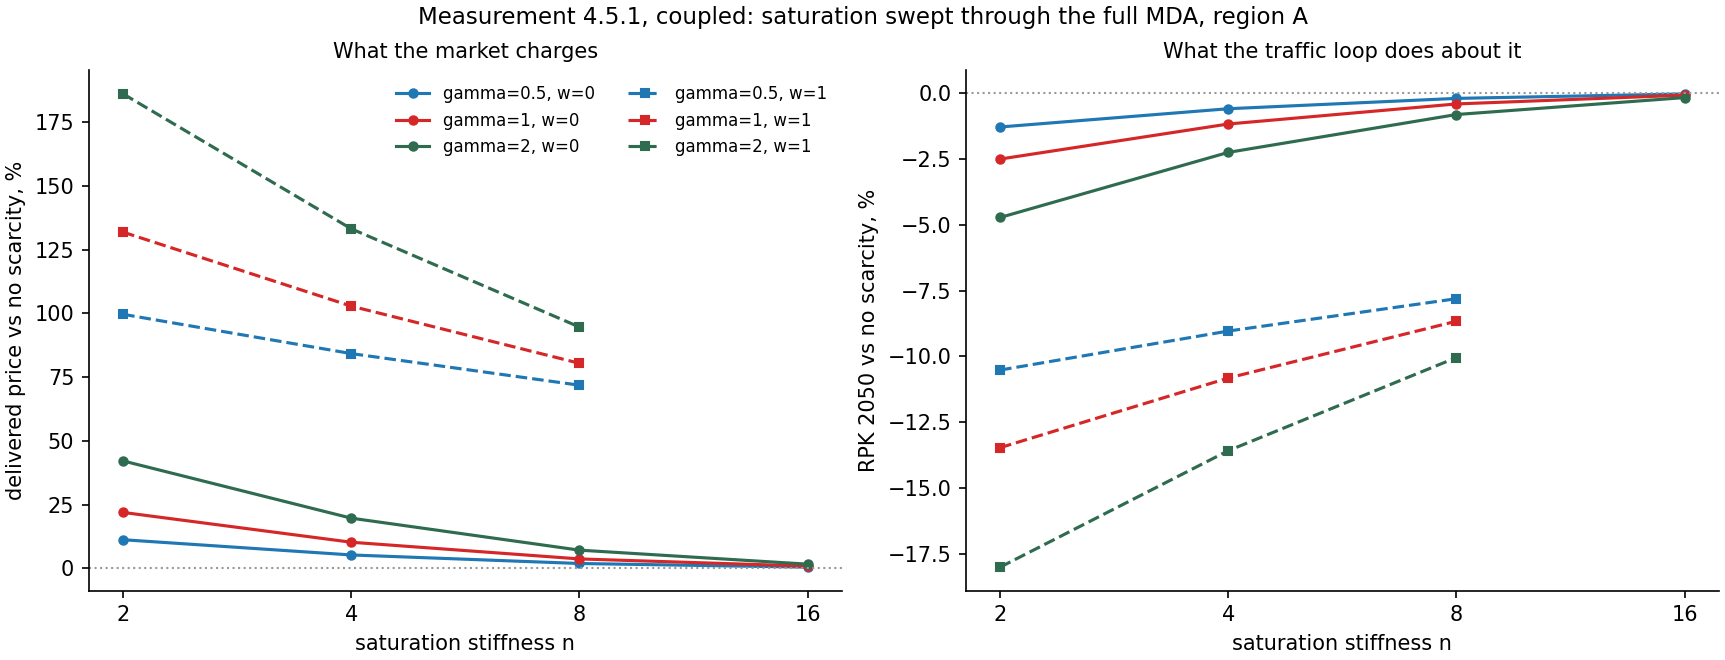
\includegraphics[width=\linewidth]{coupled_grid.png}
\caption{The same grid drawn. Gaps are cells that did not converge; they are not
interpolated over.}
\end{figure}

\noindent Two results survive the feedback intact. The kernel-level \emph{ordering} holds
--- uplift still falls monotonically in $n$. And \textbf{the traffic response is
consistently about a tenth of the price response}: $+42.1\,\%$ on price gives $-4.7\,\%$
on RPK. That ratio is the product of two independently measured transmissions (fuel is
13.1\,\% of the airfare; demand elasticity $0.888$). Rule of thumb for this bench:
\textbf{a 10\,\% fuel-price rise costs about 1.2\,\% of traffic}.

\subsection{The coupled fixed point fails at $w=1$}
\label{sec:convergence}

At $w=1$ the loop does not converge under AeroMAPS's default settings: the residual
stalls at $2.1\times10^{-1}$ after 200 iterations. Damping helps but does not close it;
acceleration fixes \emph{some} cells (3 of 12), not all.

Instrumenting per iteration locates it exactly. Everything is converged to $10^{-12}$
except \textbf{two years}, where the \emph{compliance price swings 100\,\% of its own
magnitude while the volumes move 1--2\,\%}.

\begin{keybox}
\textbf{The mechanism, and it is not ``prices are volatile''.} The measured loop gain is
$\approx 0.32$, far below 1 --- a gain that low cannot diverge. It is a
\emph{discontinuity}. A 2\,\% demand wobble flips the obligation between binding and
slack; $\lambda^{M}$ jumps between a positive value and zero when it does. The primal
barely notices; the multiplier is a step function across that boundary. The iterate
settles into an exact period-3 limit cycle.

\textbf{So $w$ decides whether the model couples to a well-defined function of its own
state.} At $w=0$ the delivered price is the \emph{average cost} --- a function of volumes,
which move 1\,\%; the jump never reaches the traffic loop and the MDA converges in 40
iterations. At $w=1$ the price contains $\lambda^{M}$, and duals at an active-set
boundary are not well-defined functions of the state.
\end{keybox}

\noindent A natural explanation was tested and \textbf{rejected}: the bad years sit next
to a ReFuelEU step, so the staircase obligation looked responsible. Replacing it with a
smooth ramp through the same points still fails. Smoothing moves the boundary rather than
removing it --- with a binding growth limit there is always some year where it stops
binding. This is intrinsic to coupling an MDA fixed point to the duals of a constrained
intertemporal programme, not a quirk of the regulation.

\textbf{Practical consequence:} $w=0$ is solid (12 of 12, default settings). $w>0$ is a
research problem, not a scenario dial, until the boundary behaviour is understood.

\section{Policy cases}
\label{sec:policy}

Five pathways --- kerosene, HEFA from waste oil, HEFA from crop oil, alcohol-to-jet,
e-fuel. \emph{Kernel-level} (Table~\ref{tab:levels}). Conclusions are about orderings and
mechanisms; the numbers are illustrative.

\subsection{Eligibility differing by region}

One ReFuelEU-like region excludes crop feedstock; the other allows it; same headline
obligation.

\begin{figure}[h]
\centering
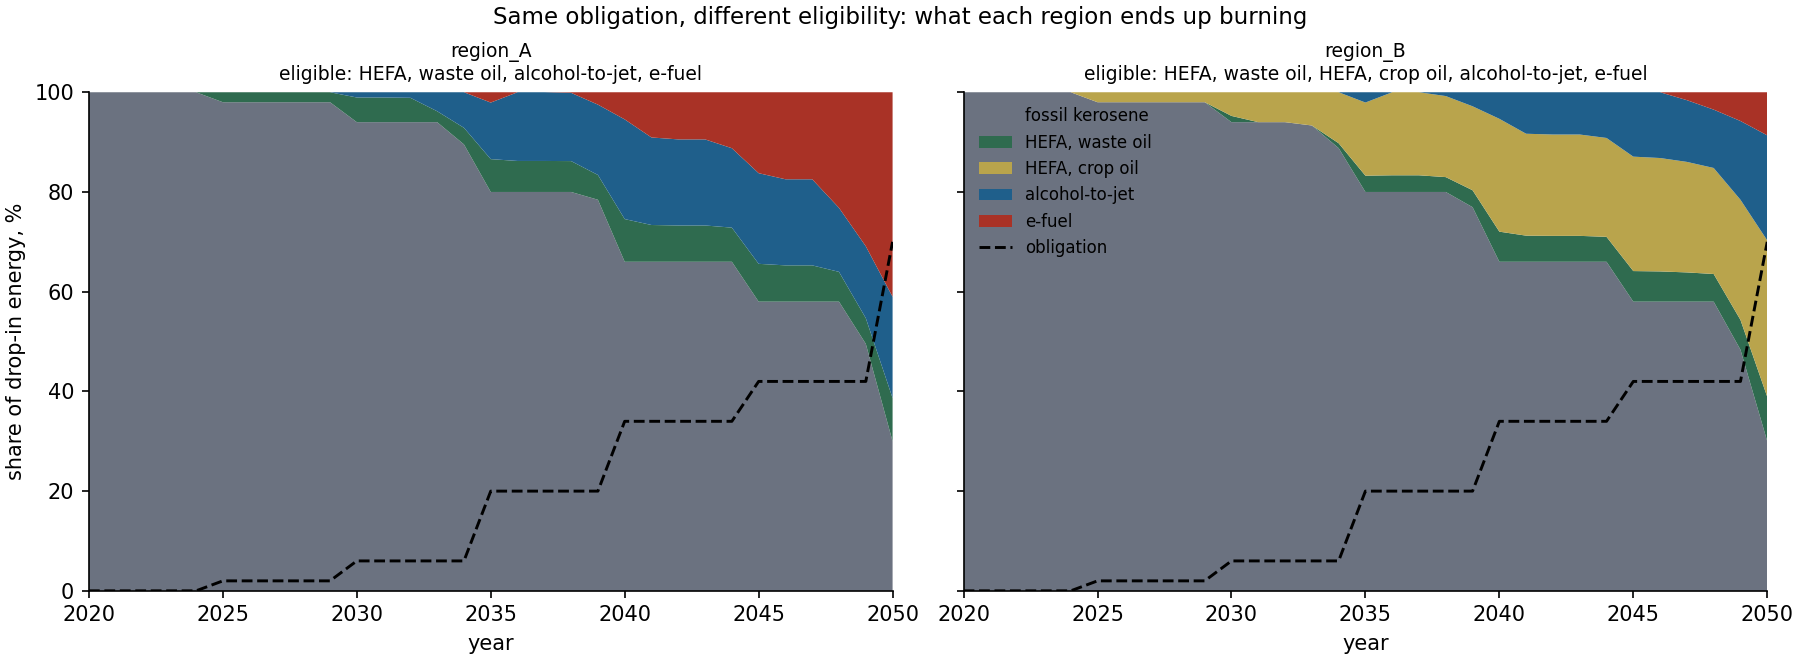
\includegraphics[width=\linewidth]{policy_fuel_mix.png}
\caption{Same target, different portfolios. The coloured band is mandated fuel; the dashed
staircase is the obligation, so colour above the line is anticipation.}
\end{figure}

\begin{keybox}
\textbf{Excluding a cheap feedstock is dearer every year except the last}: $+60\,\%$ on
the compliance price in 2030, $+139\,\%$ in 2040, and $\mathbf{-10\,\%}$ in 2050.

The mechanism is the growth limit. Denied the cheap option, region A builds e-fuel early
and arrives at 2049 with a 30.9\,\% base; the permissive region coasts on crop oil and
arrives with 5.0\,\%. When the obligation jumps 42\,\%$\to$70\,\%, all four of the
permissive region's pathways hit their growth limits at once.

\textbf{Cheap options early leave you worse placed for a steep step later} --- a result a
share-allocation model cannot produce, because it has no notion of what was built when.
\end{keybox}

\begin{figure}[h]
\centering
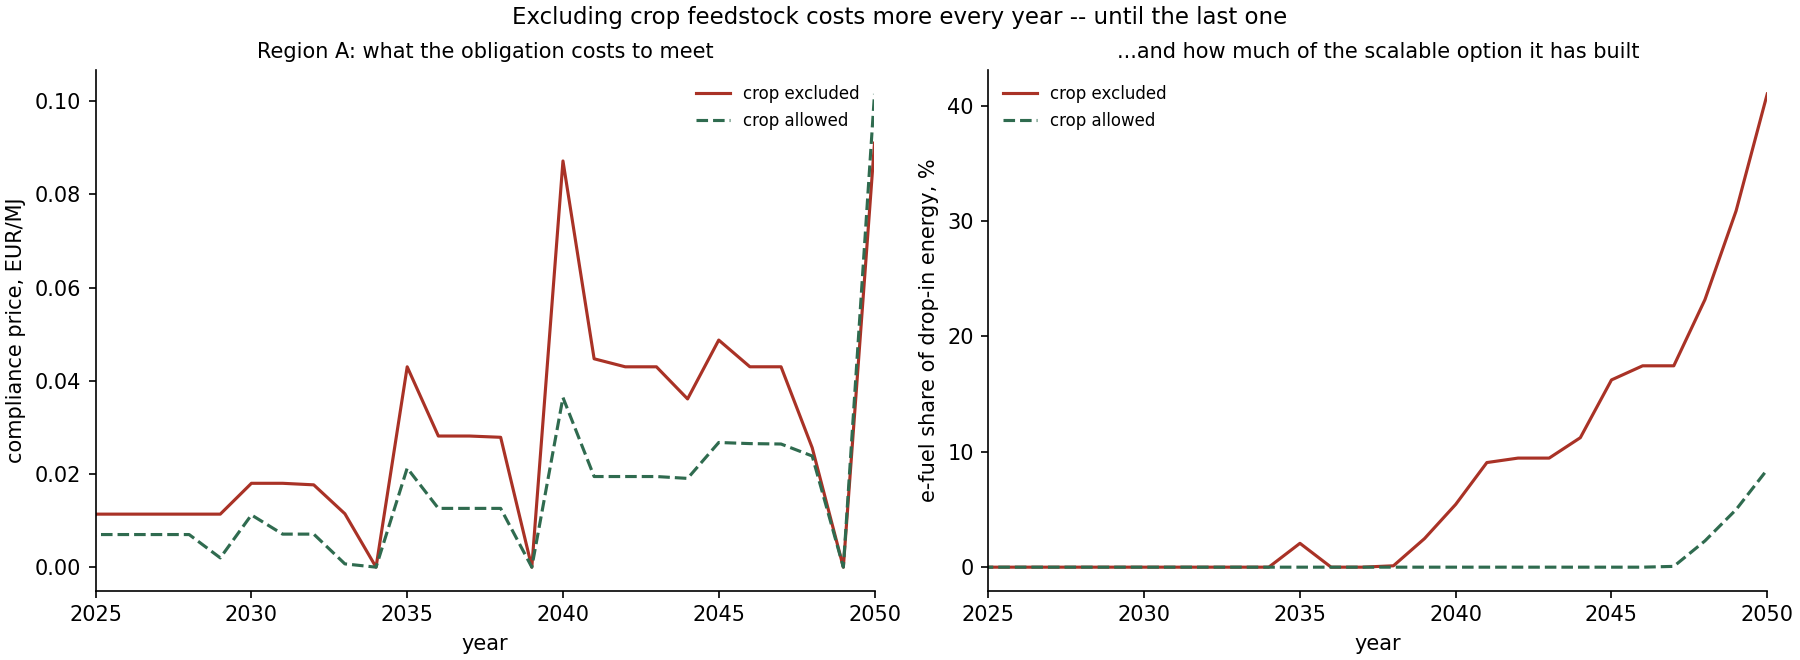
\includegraphics[width=\linewidth]{policy_exclusion_cost.png}
\caption{The cost, and the reason for it. Left: the exclusion is dearer in every year
until the last; the sawtooth is each obligation step landing and the market catching up.
Right: what it bought --- a built-out e-fuel industry.}
\end{figure}

\subsection{A sub-target within the target}

ReFuelEU's synthetic-fuel trajectory, on top of the headline obligation:

\begin{table}[h]
\centering\small
\begin{tabular}{@{}lrrr@{}}
\toprule
 & \textbf{2030} & \textbf{2040} & \textbf{2050} \\
\midrule
e-fuel, no sub-target & 0.0\,\% & 5.4\,\% & 41.0\,\% \\
e-fuel, with sub-target & 1.2\,\% & 15.0\,\% & \textbf{46.2\,\%} \\
Main compliance price & $0.01800 \to 0.01721$ & $0.08718 \to \mathbf{0.04103}$ & $0.09100 \to \mathbf{0.06908}$ \\
\bottomrule
\end{tabular}
\end{table}

\noindent By 2050 e-fuel \emph{exceeds} the 35\,\% target, because the forced early
build-out leaves a bigger base to grow from.

\begin{figure}[h]
\centering
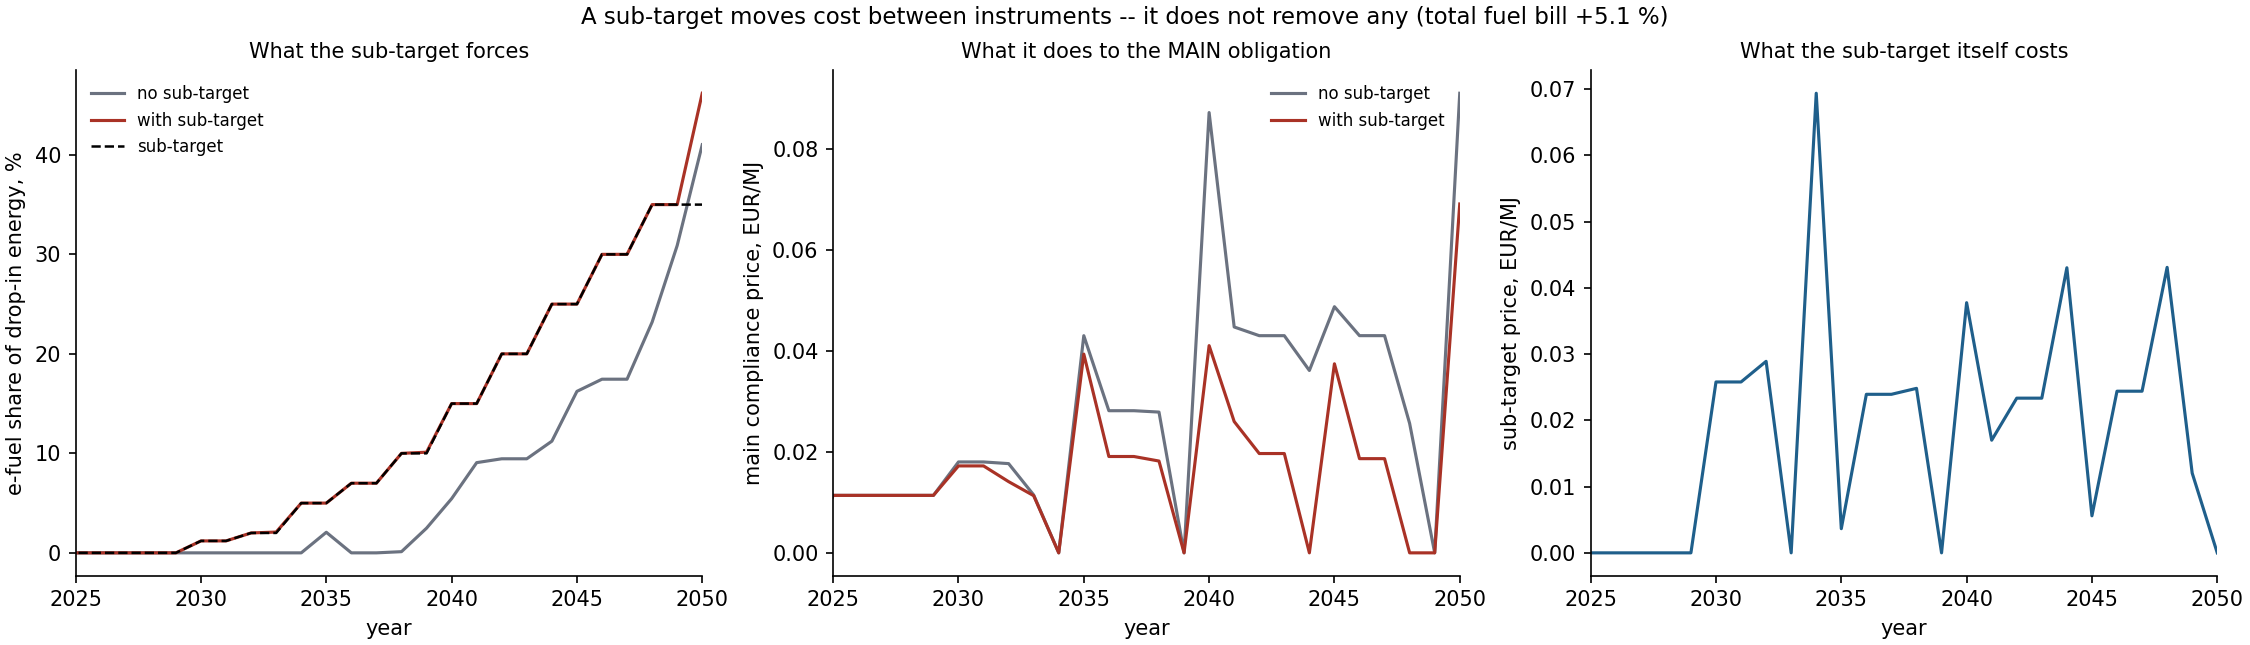
\includegraphics[width=\linewidth]{policy_submandate.png}
\caption{Left: the sub-target tracked exactly, then overshot. Middle: the headline
obligation gets cheaper throughout. Right: the sub-target's own price.}
\end{figure}

\begin{keybox}
\textbf{A number that invites the wrong conclusion.} The main compliance price falls in
every year --- by 53\,\% in 2040. That is \emph{not} the sub-target making compliance
cheaper: an extra constraint on the same programme can only make the optimum dearer, and
it does. \textbf{Total production cost $+10.7\,\%$; fuel bill $+5.1\,\%$.} What falls is
the price of \emph{one instrument} because the other is now doing that work. Quoting the
compliance price alone would show a policy paying for itself while it does the opposite.
\end{keybox}

\subsection{A carbon tax, and nothing else}

Every obligation switched off.

\begin{figure}[h]
\centering
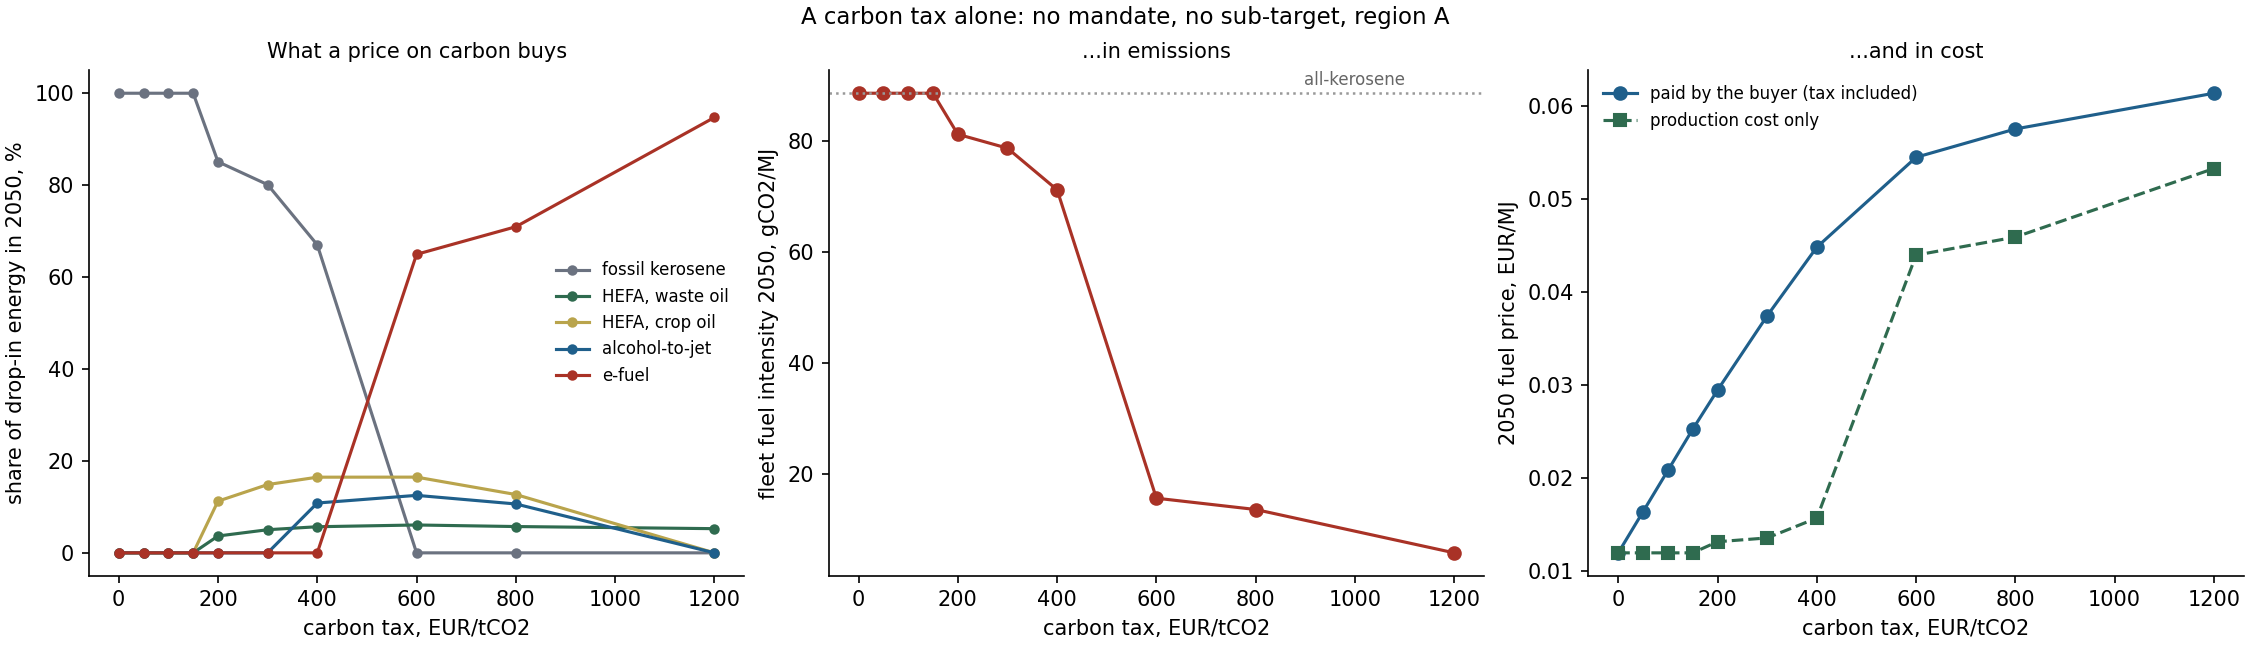
\includegraphics[width=\linewidth]{policy_carbon_tax.png}
\caption{Nothing, then everything.}
\end{figure}

\begin{keybox}
\textbf{Below about 170\,EUR/t a carbon tax on aviation fuel buys nothing at all.} The mix
stays 100\,\% kerosene and the intensity does not move from 88.6\,gCO$_2$/MJ --- it is pure
revenue.

\textbf{Then a cliff between 400 and 600}, where kerosene goes from 67\,\% to zero and
intensity falls $71.2 \to 15.7$. Not an artefact: kerosene's tax-inclusive cost
($0.0120 + 88.6\tau/10^{6}$) crosses e-fuel's ($0.0550 + 5.0\tau/10^{6}$) at
$\tau = 514$\,EUR/t, and the whole residual switches at once, because nothing
distinguishes one litre of kerosene from another. \textbf{A tax moves one crossing point
at a time, so its effect is a staircase, not a slope.}
\end{keybox}

\subsection{The same destination by two instruments}

\begin{table}[h]
\centering\small
\begin{tabular}{@{}lrrl@{}}
\toprule
\textbf{Same 70\,\% sustainable, 2050} & \textbf{Production cost} & \textbf{Intensity} & \textbf{Mix} \\
\midrule
Obligation (crop excluded) & 0.03427 & \textbf{36.5} & 41\,\% e-fuel, no crop \\
Carbon tax, 515\,EUR/t & \textbf{0.03056} & 41.3 & 33\,\% e-fuel, 18\,\% crop \\
\bottomrule
\end{tabular}
\end{table}

\noindent The tax is \textbf{10.8\,\% cheaper} and \textbf{13\,\% dirtier}: it buys the
cheapest sustainable fuel, the obligation's feedstock rule buys a cleaner one.

\begin{keybox}
\textbf{The environmental work is done by the eligibility rule, not by the volume
target.} A mandate written in volumes is not an emissions instrument. It becomes one only
through the rules about what counts.
\end{keybox}

\noindent One confound: the tax case has no obligation, so no eligibility rule applies to
it and crop oil is available. That is realistic --- eligibility rules only exist inside
mandates --- but it makes this a \emph{restricted mandate against an unrestricted tax},
not instrument against instrument at equal restriction.

\section{Defects found, and one general lesson}
\label{sec:defects}

Three defects of the \emph{same family} were found, all of them producing
plausible-looking numbers rather than errors.

\begin{enumerate}[leftmargin=*]
  \item \textbf{A price for an obligation that does not exist.} Where $m=0$,
        constraint~\eqref{eq:mandate} is implied by $q,x \ge 0$ --- redundant, so its
        multiplier is free. The solver reported up to $0.0112$\,\EURMJ, roughly the whole
        cost of kerosene, in years with no obligation.
  \item \textbf{An indeterminate split at a 100\,\% obligation.} There the obligation
        forces conventional supply to zero, so \eqref{eq:balance} and \eqref{eq:mandate}
        have the same active rows and only their \emph{sum} is determined. The solver
        split the identical problem three different ways, including a \emph{negative}
        energy price.
  \item \textbf{A jump at a binding/slack boundary} --- \S\ref{sec:convergence}. The same
        thing dynamically, and the one that stops the solver.
\end{enumerate}

\noindent In every case a constraint stopped being independent and its multiplier became
arbitrary. The first two are now pinned to their meaningful KKT values; the third is not
fixable that way, because the discontinuity is real.

\begin{keybox}
\textbf{A convex programme that \emph{solves} is not a programme that is \emph{right}.}
The saturation term was first written as $a\,q^{n+1}$ with $a = c\gamma/((n{+}1)K^{n})$
--- algebraically correct, numerically unusable: $a$ carries $K^{-n}$ and the coefficients
spanned 35 orders of magnitude at $n=16$. Half the parameter grid refused to solve; worse,
\emph{where it did solve it returned a suboptimal point}, 0.13\,\% dearer, which showed up
as a \textbf{3.4\,\% error in the delivered price} --- at the exact settings the whole
sensitivity table was built on. The solver reported \texttt{optimal} both times.

Rewriting it in the utilisation it is actually a function of,
$[c\gamma K/(n{+}1)]\,(q/K)^{n+1}$, made all 36 cells solve. The only thing that caught
the wrong answer was scoring the returned point against the objective \emph{independently
of the solver}.
\end{keybox}

\section{Limitations}

\begin{itemize}[leftmargin=*,nosep]
  \item \textbf{Regions do not interact.} Every constraint is per region and the objective
        is a plain sum, so solving jointly and separately agree to solver noise. There is
        no \textbf{leakage}: a stricter region cannot import compliance from a looser one.
        This is the single most important missing mechanism for policy work.
  \item \textbf{$w>0$ does not reliably converge} (\S\ref{sec:convergence}).
  \item \textbf{The buy-out payment reaches no one} (\S\ref{sec:whopays}).
  \item \textbf{No learning curve} anywhere in AeroMAPS, so the cost of entry is a
        constant and every price dynamic comes from the model's own scarcity terms.
  \item \textbf{Bottom-up costs are excluded ``for now''}, and not for the usual reason. A
        vintage \emph{mix} effect makes average cost \emph{fall} as volume rises, which
        makes the cost integral concave and the duals stop being prices. A loop is not the
        obstacle; the sign is.
  \item \textbf{2050 is the horizon} and also the steepest step, so results turning on
        ``what is built by the end'' are partly a terminal condition.
  \item \textbf{Emission factors and four of the five costs are assumed.}
\end{itemize}

\section{Where this goes next}

\begin{enumerate}[leftmargin=*,nosep]
  \item \textbf{Inter-regional trade}, which is what the global (non-namespaced)
        discipline was built for. At step~1 it is global in plumbing, not economics.
  \item \textbf{Understand the $w>0$ boundary behaviour}, or decide the model reports the
        rent without charging it.
  \item \textbf{Pass the buy-out payment through} to the cost chain.
  \item \textbf{Make \var{cvxpy} a proper optional dependency} before the mode ships.
\end{enumerate}

\end{document}
